% ===========================================================================
\section{Milestone IV: The CMB and matter power spectra}\label{sec:m4}
% ===========================================================================

The last milestone turns the source functions of Milestone~III into observables: the angular power spectra of the
CMB temperature and polarization, and the matter power spectrum today. We also interpret the shapes of these spectra
in terms of the physics of the earlier milestones.

\subsection{Theory}

\paragraph*{Statistics of the CMB sky.} The temperature fluctuation in direction $\hat{\bm n}$ is expanded in
spherical harmonics, $\Theta(\hat{\bm n})=\sum_{\ell m}a_{\ell m}Y_{\ell m}(\hat{\bm n})$. Multipole $\ell$ corresponds
to an angular scale $\theta\approx\pi/\ell$. The primordial fluctuations are a statistically homogeneous and
isotropic random field, so the $a_{\ell m}$ are uncorrelated and their variance depends only on $\ell$:
$\langle a_{\ell m}a^*_{\ell'm'}\rangle=\delta_{\ell\ell'}\delta_{mm'}C_\ell$. All the information in a Gaussian field is
in the power spectrum $C_\ell$. Since only $2\ell+1$ values of $m$ are available for each $\ell$, $C_\ell$ can only be
measured with a relative precision of $\sqrt{2/(2\ell+1)}$ (cosmic variance), which dominates the error bars at
low $\ell$.

The primordial curvature perturbation has the power spectrum
$\langle\mathcal{R}(\bm k)\mathcal{R}^*(\bm k')\rangle=(2\pi)^3\delta^3(\bm k-\bm k')\,2\pi^2\mathcal{P}_{\mathcal{R}}(k)/k^3$,
with $\mathcal{P}_{\mathcal{R}}=A_s(k/k_{\rm pivot})^{n_s-1}$. Inflation predicts a nearly scale-invariant spectrum,
$n_s\simeq1$, in which every logarithmic interval of $k$ contributes equally to the curvature fluctuations. Because the
evolution is linear and every mode in Milestone~III was normalized to $\mathcal{R}=1$, every observable is a
primordial amplitude times a transfer function.

\paragraph*{The line-of-sight integral.} A direct solution of the photon hierarchy up to $\ell\sim2500$ would need
thousands of coupled equations per mode. Seljak and Zaldarriaga~\cite{Seljak1996} noticed that Eq.~\eqref{eq:boltz_photon}
is a linear first-order equation in $\Theta$ that can be integrated formally. In conformal time it has the form
$\dot\Theta+(ik\mu-\dot\tau)\Theta=\tilde S$, where $\tilde S$ collects all terms that do not contain $\Theta$
itself. With the integrating factor $e^{ik\mu\eta-\tau}$ and $\tau(\eta_0)=0$,
\begin{equation}
\Theta(k,\mu,\eta_0)=\int_0^{\eta_0}\tilde S(k,\mu,\eta)\,e^{-\tau(\eta)}\,e^{-ik\mu(\eta_0-\eta)}\,\dd\eta .
\end{equation}
The temperature today is a sum of contributions emitted along the photon path, each attenuated by the probability
$e^{-\tau}$ that the photon is not scattered again. The phase factor is a plane wave, which the Rayleigh formula
$e^{-ik\mu\chi}=\sum_\ell(-i)^\ell(2\ell+1)j_\ell(k\chi)P_\ell(\mu)$ expands into spherical Bessel functions. After
integrating the $\mu$-dependent terms of the source by parts we obtain
\begin{align}
\Theta_\ell(k) &= \int_{-\infty}^{0} S_T(k,x)\,j_\ell[k(\eta_0-\eta)]\,\dd x, \label{eq:los}\\
\Theta^E_\ell(k) &= \sqrt{\frac{(\ell+2)!}{(\ell-2)!}}\int_{-\infty}^{0} S_E(k,x)\,j_\ell[k(\eta_0-\eta)]\,\dd x,
\end{align}
with the source functions of Eqs.~\eqref{eq:ST} and \eqref{eq:SE}. This separates the problem into physics
(the source $S$, which only needs the low multipoles and is smooth in $k$) and geometry (the Bessel function, which
projects a plane wave at distance $\eta_0-\eta$ onto multipole $\ell$). The function $j_\ell(z)$ peaks near $z\approx\ell$,
so a perturbation of wavenumber $k$ on the last-scattering surface at distance $\chi_*=\eta_0-\eta_*$ is seen mainly at
$\ell\approx k\chi_*$. The angular power spectra are
\begin{equation}
C_\ell^{XY} = 4\pi\int_0^\infty\frac{\dd k}{k}\,\mathcal{P}_{\mathcal{R}}(k)\,\Theta^X_\ell(k)\,\Theta^Y_\ell(k),
\label{eq:cl}
\end{equation}
with $X,Y\in\{T,E\}$. We plot $D_\ell=\ell(\ell+1)C_\ell/2\pi$ in $\mu$K$^2$, multiplying by $(10^6T_{\rm CMB})^2$;
$D_\ell$ is the variance of the temperature per logarithmic interval in $\ell$.

\paragraph*{The Sachs--Wolfe plateau.} On scales larger than the sound horizon at decoupling the photons have not
oscillated, and only the SW term contributes, $\Theta_\ell\approx(\Theta_0+\Psi)(k,\eta_*)\,j_\ell(k\chi_*)$. In MD the
adiabatic initial conditions give $\Theta_0=-\tfrac23\Psi$, so the observed temperature is $\Theta_0+\Psi=\Psi/3$: the
photons from a potential well start out hotter, but lose more energy climbing out. With $\Psi=-\tfrac35\mathcal{R}$,
$\Theta_0+\Psi=-\mathcal{R}/5$. Using $\int_0^\infty j_\ell^2(z)\,\dd z/z=1/[2\ell(\ell+1)]$ we find, for $n_s=1$,
\begin{equation}
D_\ell^{\rm SW} = \frac{A_s}{25}T_{\rm CMB}^2 \approx 620\muK,
\label{eq:SWplateau}
\end{equation}
independent of $\ell$. A scale-invariant primordial spectrum gives a flat $D_\ell$ on large scales.

\paragraph*{Acoustic peaks.} On smaller scales the SW term is the acoustic oscillation of Eq.~\eqref{eq:acoustic},
frozen at decoupling, $\Theta_0+\Psi\propto\cos(kr_{s*})$. Modes that are at an extremum at decoupling,
$k_nr_{s*}=n\pi$, give peaks in the spectrum. They project to
\begin{equation}
\ell_n\approx n\,\ell_A - \phi_n,\qquad \ell_A=\frac{\pi\chi_*}{r_{s*}},
\label{eq:lA}
\end{equation}
where $\phi_n$ is a phase shift caused by the driving potentials and by the projection. Odd peaks ($n=1,3,\dots$) are
compressions in potential wells and even peaks are rarefactions. The Doppler term $\propto v_b\propto\sin(kr_s)$ is
out of phase with the density and fills in the troughs between the peaks. On small scales diffusion damping suppresses
the power by $\sim e^{-2(\ell/\ell_D)^2}$, with $\ell_D=k_D\chi_*$.

\paragraph*{The matter power spectrum.} The matter power spectrum follows from $\Phi$ through the Poisson equation.
We use the comoving-gauge density contrast, which is the gauge-invariant quantity that reduces to the Newtonian density
contrast inside the horizon (in the code we evaluate it directly as
$\sum_i\rho_i[\delta_i-3\Hp v_i/(ck)]/\sum_i\rho_i$ for CDM and baryons, which is the same up to radiation terms of
order $10^{-3}$ on the largest scales; Sec.~\ref{sec:neutrinos}),
\begin{equation}
\Delta_M(k,x) = \frac{2}{3}\frac{c^2k^2}{\Hp^2}\frac{\Phi(k,x)}{\Om_M(x)},
\label{eq:DeltaM}
\end{equation}
and $P(k,x)=|\Delta_M(k,x)|^2\,2\pi^2\mathcal{P}_{\mathcal{R}}(k)/k^3$. Its shape follows from Milestone~III:
\begin{itemize}
\item For $k\ll k_{\rm eq}$ the mode entered during MD, $\Phi$ is constant and the same for all such $k$. Then
      $\Delta_M\propto k^2$ and $P\propto k^4\mathcal{P}_{\mathcal{R}}/k^3\propto k^{n_s}$.
\item For $k\gg k_{\rm eq}$ the potential decayed in RD by $\sim(k_{\rm eq}/k)^2$, partly compensated by the
      logarithmic M\'esz\'aros growth. This gives $P\propto k^{n_s-4}\ln^2(k/k_{\rm eq})$.
\end{itemize}
The spectrum therefore peaks near $k_{\rm eq}$. Because $k_{\rm eq}\propto\Om_{M0}h^2$ in units of Mpc$^{-1}$, the
peak position measures the matter density.

\subsection{Implementation and tests}

\texttt{PowerSpectrum} first tabulates $j_\ell(z)$ for all needed $\ell$ on a uniform grid with 32 points per
$2\pi$, and $j_\ell(z)/z^2$ for the $E$-mode source of Eq.~\eqref{eq:SE}. Uniform grids allow $O(1)$ spline lookups.
We evaluate Eq.~\eqref{eq:los} by the trapezoidal rule on an $x$-grid that starts at $x=-8.5$, when $e^{-\tau}$ makes
the source negligible. The grid has spacing $\Delta x=0.003$ around recombination, to resolve $\gt$, and is uniform in
$\eta$ elsewhere, with five points per Bessel oscillation at $k_{\max}$. The $k$-integral uses four points per period
$2\pi/\eta_0$ of the transfer functions (and $\Delta\ln k\le0.02$ at small $k$), up to $k_{\max}=0.3\Mpc^{-1}$, i.e.\
$k\eta_0\approx4300$. We compute $C_\ell$ at 97 multipoles between 2 and 2500 and spline in $\ell$. The full run
(background, recombination, perturbations and spectra) takes about 60\,s on two cores.

Tests include:
\begin{itemize}
\item The SW term alone gives the plateau of Eq.~\eqref{eq:SWplateau} at low $\ell$, corrected for the effects
      discussed below.
\item The peak spacing agrees with $\ell_A$ from the sound horizon and $\chi_*$.
\item $C_\ell^{EE}\ge0$ and $|C_\ell^{TE}|\le\sqrt{C_\ell^{TT}C_\ell^{EE}}$.
\item Doubling the LOS and $k$ sampling changes the spectra by less than $5\times10^{-5}$.
\item $P(k)$ has slope $n_s$ at small $k$ and turns over at $k_{\rm eq}$.
\end{itemize}

\subsection{Results}

\begin{figure}
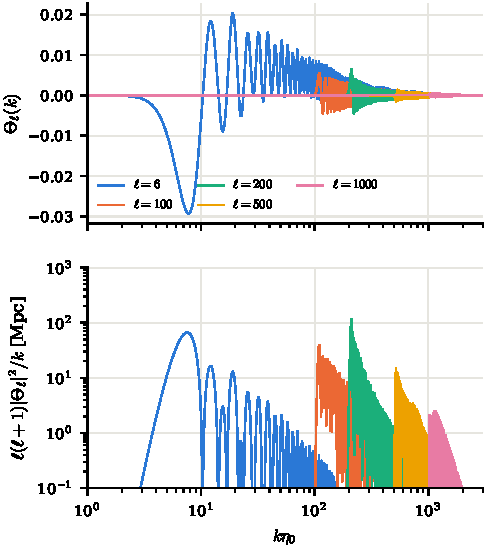
\includegraphics[width=\columnwidth]{m4_transfer}
\caption{Photon transfer functions $\Theta_\ell(k)$ (\emph{top}) and the integrand $\ell(\ell+1)\Theta_\ell^2/k$ of
$C_\ell$ (\emph{bottom}) for $\ell=6$, 100, 200, 500 and 1000, as functions of $k\eta_0$.}
\label{fig:transfer}
\end{figure}

\paragraph*{Transfer functions.} Figure~\ref{fig:transfer} shows the projection at work. $\Theta_\ell(k)$ is zero for
$k\eta_0<\ell$, where $j_\ell$ vanishes: a wave cannot produce structure on angles smaller than its own projected
wavelength. It peaks at $k\eta_0\simeq\ell$ (more precisely $k\chi_*\simeq\ell$), where the wave vector is
perpendicular to the line of sight. It then oscillates with a slowly decaying tail from waves whose wave vector is
inclined to the line of sight; their crests are farther apart on the sky, so they project onto larger angles. Each
multipole therefore receives contributions from a range of $k$, which smears the acoustic features: the peaks in $C_\ell$
are much broader than the oscillations of $\Theta_0(k)$ at recombination. The integrand of $C_\ell$ (bottom panel) is
dominated by the first peak at $k\chi_*\approx\ell$. Its height follows the acoustic oscillations: $\ell=200$ sits on
the first peak and has a much larger integrand than $\ell=100$, while $\ell=1000$ is suppressed by damping.

\begin{figure}
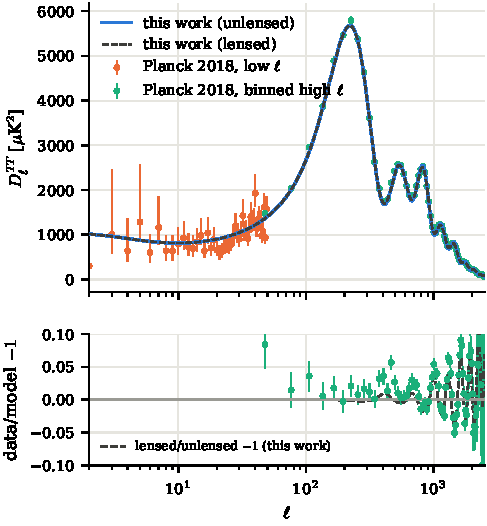
\includegraphics[width=\columnwidth]{m4_TT_planck}
\caption{\emph{Top:} our TT spectrum, unlensed and lensed, compared with Planck 2018 data~\cite{Planck2018spectra}:
the low-$\ell$ spectrum with asymmetric error bars and the binned high-$\ell$ spectrum. \emph{Bottom:} residuals of the
high-$\ell$ data relative to our unlensed model. The dashed line is our own lensed/unlensed ratio minus one
(Sec.~\ref{sec:lensing}), which follows the oscillating residuals.}
\label{fig:TT}
\end{figure}

\paragraph*{The temperature spectrum.} Figure~\ref{fig:TT} compares our TT spectrum with Planck. The model reproduces the
Sachs--Wolfe plateau, the positions of the seven acoustic peaks visible in the data, and the damping tail. The main
features have the following physical explanation:
\begin{itemize}
\item \emph{Plateau.} At $\ell=10$, $D_\ell=815\muK$, higher than the estimate $620\muK$ of
      Eq.~\eqref{eq:SWplateau}. Two effects account for most of the difference. First, at decoupling radiation still
      makes up $24\%$ of the density, so the largest modes have $\Theta_0+\Psi=-0.236$ instead of the MD value $-0.2$.
      Second, the red tilt $n_s<1$ gives more power at $k\sim\ell/\chi_*\ll k_{\rm pivot}$, a factor $1.16$ at
      $\ell=10$. Reionization lowers the plateau only marginally, since the scales it affects are smaller.
\item \emph{Peak positions.} The first peak is at $\ell=221$ and the next ones at $\ell=538$, 817, 1133, 1432, 1745 and
      2046. Their spacing, $\approx300$, agrees with $\ell_A=\pi\chi_*/r_{s*}=303$ for $\chi_*=13\,911\Mpc$ and
      $r_{s*}=144.4\Mpc$. The angular size of the sound horizon at last scattering is thus about $0.6^\circ$. The first
      peak lies at $\approx0.73\,\ell_A$ because of the phase shift from the decaying potentials. The peak positions
      measure the angle $r_{s*}/\chi_*$: in a curved universe the same ruler would appear at a different angle, so the
      peak positions are the CMB's main constraint on spatial curvature.
\item \emph{Peak heights.} The first peak is boosted by radiation driving. The second peak (a rarefaction) is lower
      than the first and third relative to a smooth envelope, because the baryons shift the zero point of the
      oscillation towards compression. The ratio of odd to even peaks measures $\Om_bh^2$.
\item \emph{Damping tail.} Above $\ell\sim1000$ the power falls steeply. From Eq.~\eqref{eq:silk} we find
      $k_D=0.14\Mpc^{-1}$ at decoupling, i.e.\ $\ell_D=k_D\chi_*\approx2000$. The finite thickness of the
      last-scattering surface ($\approx40\Mpc$, Sec.~\ref{sec:m2}) adds to the suppression, since fluctuations smaller
      than the thickness average out along the line of sight.
\end{itemize}
The fiducial parameters are not fitted to the data, and the residuals are at the few-percent level. Against the 83
binned high-$\ell$ points we find $\chi^2=780.7$. The residuals oscillate for $\ell\gtrsim1000$: the data are above
the model in the troughs and below it at the peaks. This is the signature of weak gravitational lensing by
large-scale structure~\cite{Lewis2006}. The deflections of CMB photons are only $\sim2'$, but they are coherent over
degrees and remap the temperature field. In harmonic space this convolves the spectrum with the lensing kernel, which
smooths the acoustic peaks and moves power into the troughs and the damping tail. With lensing included
(Sec.~\ref{sec:lensing}) we find $\chi^2=220.2$ for the same 83 bins. Most of the residual mismatch of the unlensed
model is therefore lensing; the remainder comes from the parameters, which are not the best fit, and from the
simple recombination model.

\paragraph*{Gravitational lensing.}\label{sec:lensing}
Photons from the last-scattering surface are deflected by the gravitational potentials of the intervening structure.
To first order the observed temperature in direction $\hat{\mathbf n}$ is the unlensed one at
$\hat{\mathbf n}+\nabla\phi$, where the lensing potential is a projection of the Weyl potential $\Psi-\Phi$ (the
combination that bends light, since both potentials contribute to the null geodesic),
\begin{equation}
\phi(\hat{\mathbf n})=-\int_0^{\chi_*}\!d\chi\,\frac{r(\chi_*-\chi)}{r(\chi_*)\,r(\chi)}\,
\bigl(\Psi-\Phi\bigr)\bigl(\chi\hat{\mathbf n},\eta_0-\chi\bigr),
\label{eq:phi}
\end{equation}
with $r(\chi)$ the comoving angular distance ($r=\chi$ when flat; Sec.~\ref{sec:curvature}). The geometric kernel
peaks halfway to the source, so lenses at $z\sim2$ dominate. We treat the last-scattering surface as a single source
plane at the peak of the visibility function. $C_\ell^{\phi\phi}$ follows from the same line-of-sight machinery as
the temperature, with source~\eqref{eq:phi}, for $\ell<30$; above that we use the Limber approximation
$C_\ell^{\phi\phi}\simeq\int d\chi\,W^2(\chi)\,P_{\Psi-\Phi}\bigl((\ell+\tfrac12)/r(\chi),\chi\bigr)/r^2(\chi)$, which
avoids integrating to large $k$ (the Weyl potential is extrapolated beyond our $k_{\max}$ as $\ln k/k^2$, its
asymptotic form in the radiation-to-matter transfer function). The two agree to $0.2\%$ at $40\le\ell\le200$.
$[\ell(\ell+1)]^2C_\ell^{\phi\phi}/2\pi$ peaks at $\ell=34$ with value
$1.41\times10^{-7}$, and the rms deflection is $2.5'$ (Fig.~\ref{fig:lensing}).

Because the deflections are small but coherent over degrees, we lens the spectra with the full-sky
correlation-function method of Challinor and Lewis~\cite{Challinor2005}, as implemented in CLASS. The lensed
correlation function is the unlensed one evaluated with the deflection field averaged over: e.g.\ for temperature
$\tilde\xi(\beta)=\sum_\ell\frac{2\ell+1}{4\pi}C_\ell\,e^{-\ell(\ell+1)\sigma^2(\beta)/2}\,d^\ell_{00}(\beta)+\dots$,
where $\sigma^2(\beta)$ is the variance of the relative deflection of two points separated by $\beta$ and the dots are
terms of first and second order in the anisotropic part $C_{{\rm gl},2}(\beta)$ of the deflection correlation. The
Gaussian factor is exact for Gaussian deflections; only the anisotropic part is expanded. Polarization uses the
spin-2 correlation functions $\xi_\pm$ and $\xi_\times$ with the Wigner functions $d^\ell_{22}$, $d^\ell_{2-2}$,
$d^\ell_{20}$, which we compute by the three-term recurrence in $\ell$. The lensed spectra follow by Gauss--Legendre
integration over $\cos\beta$. Since lensing couples multipoles over $\Delta\ell\sim$ a few hundred, the unlensed
spectra are computed to $\ell_{\max}+500$.

The effects are those of a remapping of the sky (Fig.~\ref{fig:TT}). The acoustic peaks are smoothed: at $\ell=1000$
(a trough) the power rises by $3.4\%$ and at the fifth peak ($\ell=1500$) it drops by $2.8\%$, while scales larger
than the coherence of the deflections ($\ell\lesssim200$) change by less than $0.1\%$. In the damping tail lensing
transfers power from larger scales, $+7\%$ at $\ell=2500$. The total variance $\sum(2\ell+1)C_\ell$ is almost
unchanged. The deflections also distort the E-mode pattern without respecting its parity, creating B modes from pure
E: $D_\ell^{BB}$ rises to $0.094\,\muK$ at $\ell\approx900$, with an almost white
$C_\ell^{BB}$ at low $\ell$ (Fig.~\ref{fig:lensing}). This lensing B-mode is a foreground for primordial
gravitational waves and has been measured by several experiments.

\begin{figure}
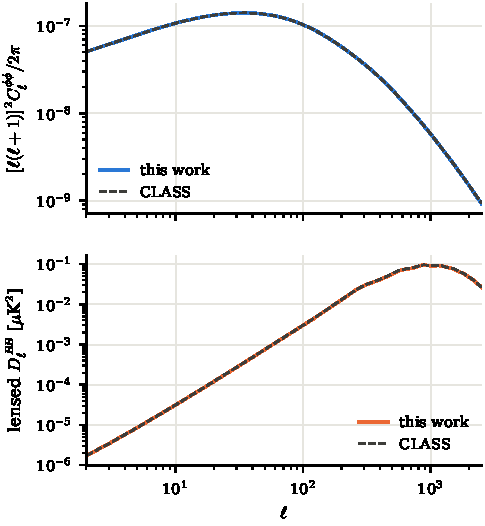
\includegraphics[width=\columnwidth]{m4_lensing}
\caption{\emph{Top:} lensing potential power spectrum. \emph{Bottom:} B-mode spectrum generated by lensing of the E
modes (no primordial B modes). Dashed: CLASS run with the same parameters.}
\label{fig:lensing}
\end{figure}

\begin{figure}
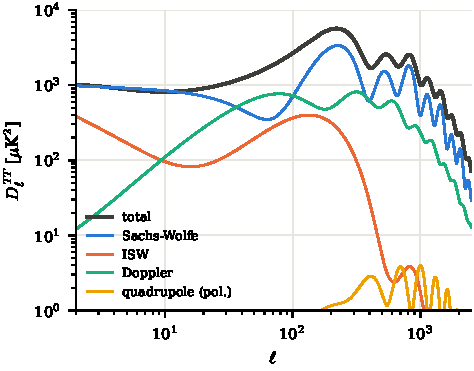
\includegraphics[width=\columnwidth]{m4_TT_components}
\caption{Contributions to the TT spectrum from the four terms of the source function~\eqref{eq:ST}, each computed
alone. They add in amplitude, not in power, so the cross terms make the total differ from the sum of the curves.}
\label{fig:TTcomp}
\end{figure}

\paragraph*{Decomposition.} Figure~\ref{fig:TTcomp} splits the TT spectrum into the four terms of Eq.~\eqref{eq:ST}:
\begin{itemize}
\item The SW term, $\Theta_0+\Psi$ at last scattering, dominates on all scales. It gives the plateau
      ($843\muK$ at $\ell=10$) and the acoustic peaks.
\item The Doppler term, from the baryon velocity at last scattering, is out of phase with the density by $\pi/2$. It
      fills in the troughs: at $\ell=400$ it is as large as the SW term. Its amplitude is reduced relative to the
      density term by $\sqrt{3}c_s/c=(1+R_b)^{-1/2}$, so the peaks remain visible. On the largest scales it vanishes,
      because the velocity is $\propto\kappa$ outside the horizon.
\item The ISW term has two parts:
      \begin{itemize}
      \item The early ISW effect comes from the potentials still decaying just after recombination, because radiation
            is not yet negligible. It adds power near the first peak ($270\muK$ at $\ell=220$), and since it adds
            coherently with the SW term, it raises the first peak considerably.
      \item The late ISW effect comes from the decay of $\Phi$ in the $\Lambda$ era. A photon crossing a decaying
            potential well gains more energy falling in than it loses climbing out. The potentials decay only on very
            large scales today, so the late ISW dominates the rise at the lowest multipoles ($385\muK$ at $\ell=2$). It is
            a direct signature of dark energy.
      \end{itemize}
\item The polarization/quadrupole term is very small, $\sim10^{-3}$ of the total.
\end{itemize}

\begin{figure}
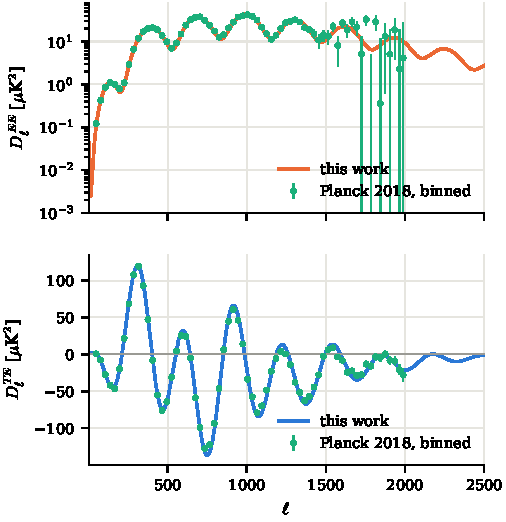
\includegraphics[width=\columnwidth]{m4_EE_TE}
\caption{$E$-mode polarization (\emph{top}) and temperature--polarization cross spectrum (\emph{bottom}) compared with
binned Planck 2018 data.}
\label{fig:EETE}
\end{figure}

\paragraph*{Polarization.} The EE and TE spectra (Fig.~\ref{fig:EETE}) agree well with Planck. Their shapes follow from
the fact that polarization is created by the quadrupole during the brief decoupling, $\Pi\propto(\kappa/\tau')\Theta_1$
(Sec.~\ref{sec:m3}):
\begin{itemize}
\item The $E$-mode peaks at $\ell=395$, 690, 994 and 1304 lie between the temperature peaks, close to the TT
      troughs, because they trace the velocity $\propto\sin(kr_s)$ rather than the density $\propto\cos(kr_s)$.
\item The EE amplitude grows from large to small scales up to $\ell\approx1000$, because the quadrupole is generated
      by free streaming over one mean free path, which is more effective for short wavelengths ($\propto k$). It then
      falls with the damping. The EE peaks are about 100 times lower than the TT peaks.
\item At $\ell\lesssim10$ the reionization bump ($D_\ell\approx0.04\muK$) comes from rescattering at $z\lesssim10$.
      The relevant quadrupole is the large-scale temperature anisotropy seen by the free electrons at reionization,
      and the horizon at $z=8$ projects to $\ell\sim$ a few. The amplitude scales as $\tau_{\rm reion}^2$, so this bump is
      the main handle on reionization.
\item The TE spectrum correlates the density and velocity terms, $\propto\cos(kr_s)\sin(kr_s)\propto\sin(2kr_s)$. It
      therefore changes sign twice as often as the TT peaks repeat: at $\ell=52$, 211, 401, 550, \dots. Its largest
      values are $+120\muK$ at $\ell=310$ and $-137\muK$ at $\ell=751$. The anti-correlation at $\ell\sim50$--$200$, on
      scales larger than the sound horizon, is a key signature that the fluctuations were adiabatic and present
      before they entered the horizon, as inflation predicts.
\end{itemize}

\begin{figure}
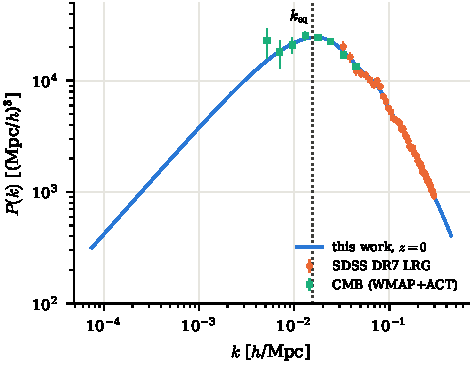
\includegraphics[width=\columnwidth]{m4_Pk}
\caption{Matter power spectrum today compared with the SDSS DR7 luminous red galaxy power spectrum~\cite{Reid2010} and
with the estimate from WMAP and ACT CMB data. The vertical dotted line marks $k_{\rm eq}$.}
\label{fig:Pk}
\end{figure}

\paragraph*{Matter power spectrum.} The matter power spectrum (Fig.~\ref{fig:Pk}) peaks at $k=0.0167\hMpc$ with
$P=2.46\times10^4\,(h^{-1}\Mpc)^3$, close to $k_{\rm eq}=0.0155\hMpc$ from Milestone~I. On large scales the slope is
$0.95\approx n_s$, the primordial spectrum. On small scales the spectrum falls as modes that entered during RD were
suppressed. Between $0.1$ and $0.4\hMpc$ the local slope is $-1.7$; the asymptotic $k^{n_s-4}\ln^2k$ is only reached at
much larger $k$. The peak is not sharp, because the transition from RD to MD is gradual.

The baryon acoustic oscillations appear as small wiggles at $k\sim0.05$--$0.3\hMpc$, with period
$2\pi/r_s(z_d)\approx0.064\hMpc$. They are the same sound waves as in the CMB, frozen into the baryon distribution at
the drag epoch, and then imprinted in the dark matter as the baryons fell into the dark matter wells. Their amplitude is
small because the baryons are only $16\%$ of the matter.

The model matches the CMB-derived points and the SDSS DR7 LRG spectrum, with $\chi^2=12.2$ for the 45 LRG points
(compared directly, without a free bias or amplitude parameter). The LRG data cover the turnover only partially, but
they clearly favour the decline at $k>k_{\rm eq}$ predicted by a universe dominated by cold dark matter. In a
baryon-only universe there would be no turnover near $k_{\rm eq}$ of this form, and the BAO wiggles would be large.

\begin{figure*}
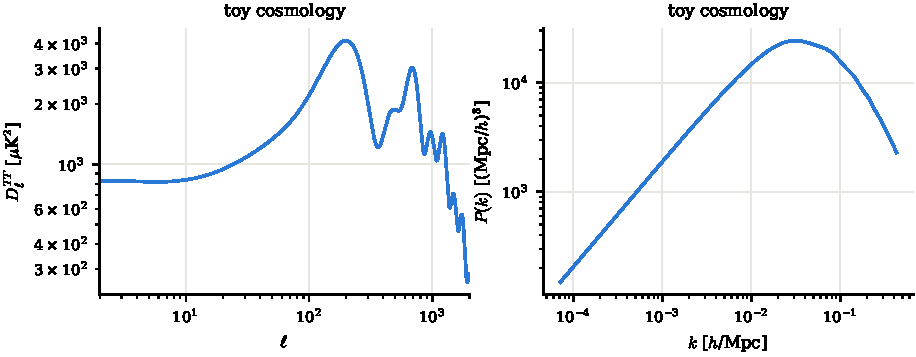
\includegraphics[width=\textwidth]{m4_toy}
\caption{TT spectrum (\emph{left}) and matter power spectrum (\emph{right}) for the toy cosmology of the course
reference figures ($h=0.7$, $\Om_b=0.05$, $\Om_{\rm CDM}=0.45$, $\Om_\Lambda=0.5$, no neutrinos, no helium, no
reionization, no polarization).}
\label{fig:toy}
\end{figure*}

\paragraph*{Toy cosmology.} As a cross-check with the reference figures of the course, we also ran a matter-heavy toy
model (Fig.~\ref{fig:toy}). The TT peaks are at $\ell=199$, 485 and 685, compared with $\approx199$, 491 and 690 read off
the reference figure. The differences from the fiducial model are what the physics above predicts:
\begin{itemize}
\item With $\Om_M=0.5$ and no neutrinos, equality is at $z\approx9900$ instead of 3400. The potentials have decayed
      less by recombination, so radiation driving and the early ISW effect are weaker.
\item The baryon loading term then dominates the peak heights, and the third peak is much higher than the second.
\item The peaks shift to lower $\ell$ because the larger matter density reduces the distance to the last-scattering
      surface ($\chi_*\approx11\,090\Mpc$, $20\%$ less) more than the sound horizon ($136\Mpc$, $6\%$ less), so
      $\ell_A\approx256$ instead of 303.
\item $P(k)$ peaks at $k=0.031\hMpc$, as expected from $k_{\rm eq}\propto\Om_M/\sqrt{\Om_r}$ in units of $h$/Mpc,
      which is larger by a factor 2.1.
\end{itemize}
The overall amplitude of both $C_\ell$ and $P(k)$ is a constant factor $\approx2.1$ higher than the reference. A constant
factor in both spectra is what a different $A_s$ would give, and the factor is consistent with the reference using
$A_s=10^{-9}$ (this is our inference; the reference does not state $A_s$).
